\subsection{Raw Audio Waveforms}\label{sec:raw_audio}
Physical acoustic waves are recorded by microphones, translating mechanincal vibrations to electrical signals, which can be stored to waveform files.
The Focus is here only on the raw waveform files and its data.
First it is to mention that waveform files are stored in some kind of audio format, e.g. .wav files, using parameters such as bit resolution, e.g. 32 bit floating point, and most importantly a sample rates $f_s$. 
The sample rate tells, which frequency range of the continuous acoustic waves form is possible to store in a discrete representation.
This is restricted by the Nyquist-Shannon sampling theorem, where the maximal frequency of the signal should not be larger than the half of the sampling frequency, otherwise aliasing effects occur. 
Thats why a usual CD format has a sampling frequency of 44.1kHz resulting in a maximum frequency of 22.05kHz, and usually humans do not hear above 20kHz frequencies.
However it is also possible to go far beyong those 44.1kHz, as it is used in telephone systems with a sampling rate of 8kHz.
This is because, voice does not need that high sampling frequency to be understandable and with enough quality.
The audio files of the speech command dataset are recorded with a sampling rate of 16kHz, which is totally enough for human speech.
Further those audio files in the speech command dataset have a time length of 1s.
The author recorded his own speech commands with one example of each command shown in \rfig{raw_audio_my}.

\begin{figure}[!ht]
  \centering
    %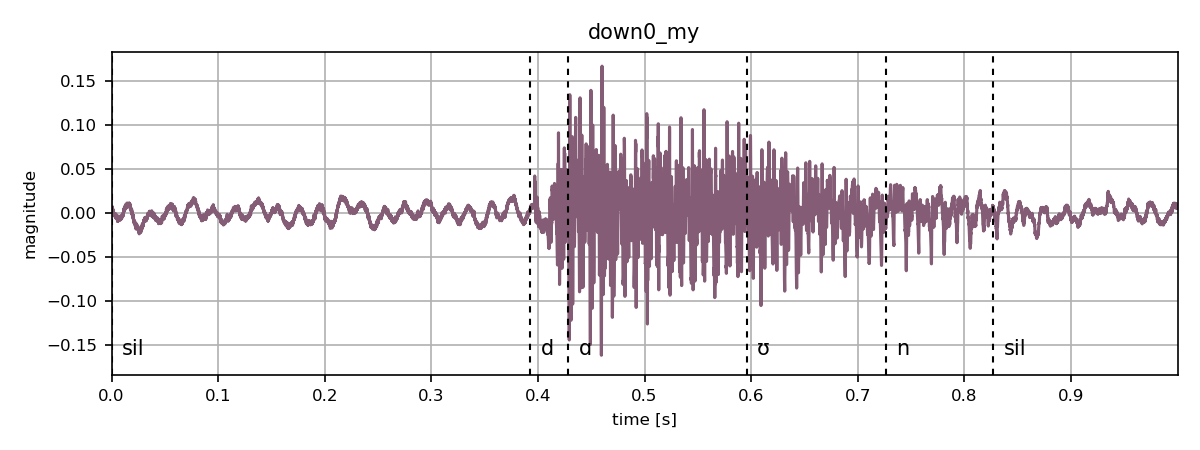
\includegraphics[width=0.65\textwidth]{./3_theory/figs/a1_raw/raw_down0_my}
    \subfigure[left]{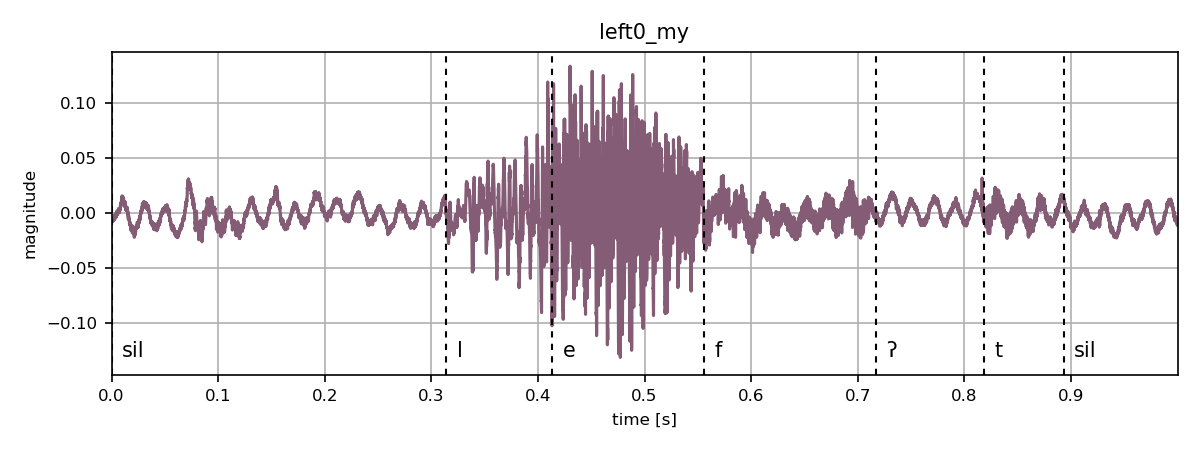
\includegraphics[width=0.45\textwidth]{./3_theory/figs/a1_raw/raw_left0_my}}
    \subfigure[right]{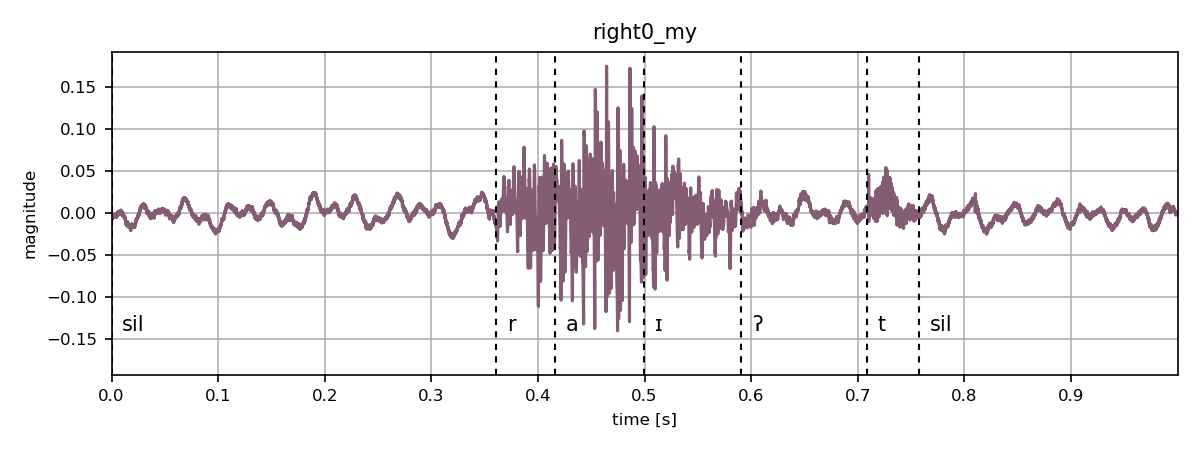
\includegraphics[width=0.45\textwidth]{./3_theory/figs/a1_raw/raw_right0_my}}
    \subfigure[up]{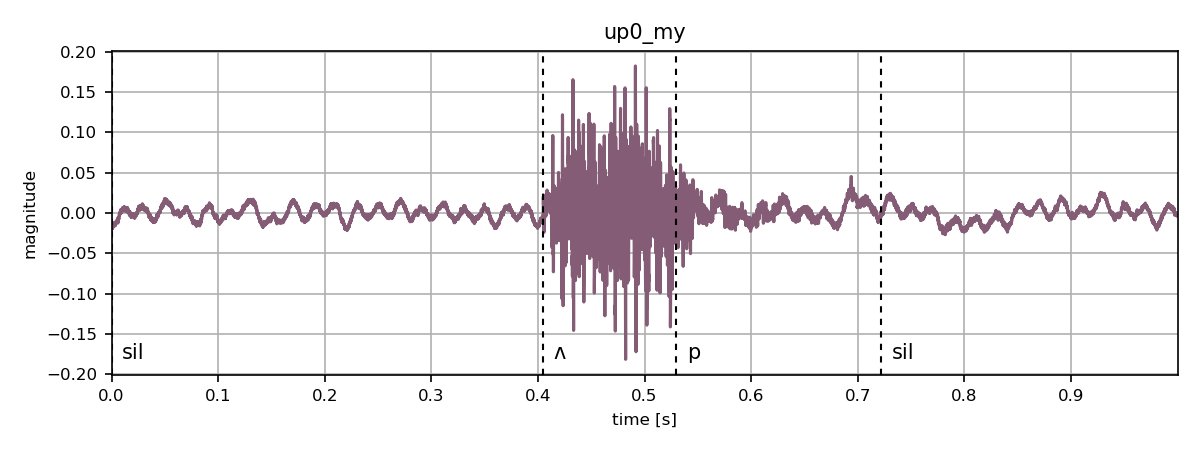
\includegraphics[width=0.45\textwidth]{./3_theory/figs/a1_raw/raw_up0_my}}
    \subfigure[down]{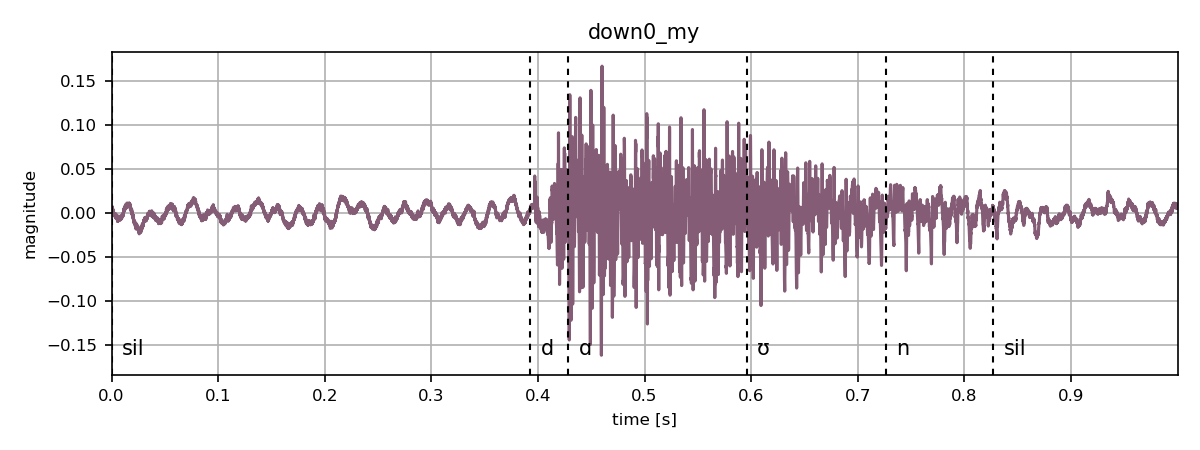
\includegraphics[width=0.45\textwidth]{./3_theory/figs/a1_raw/raw_down0_my}}
    \subfigure[go]{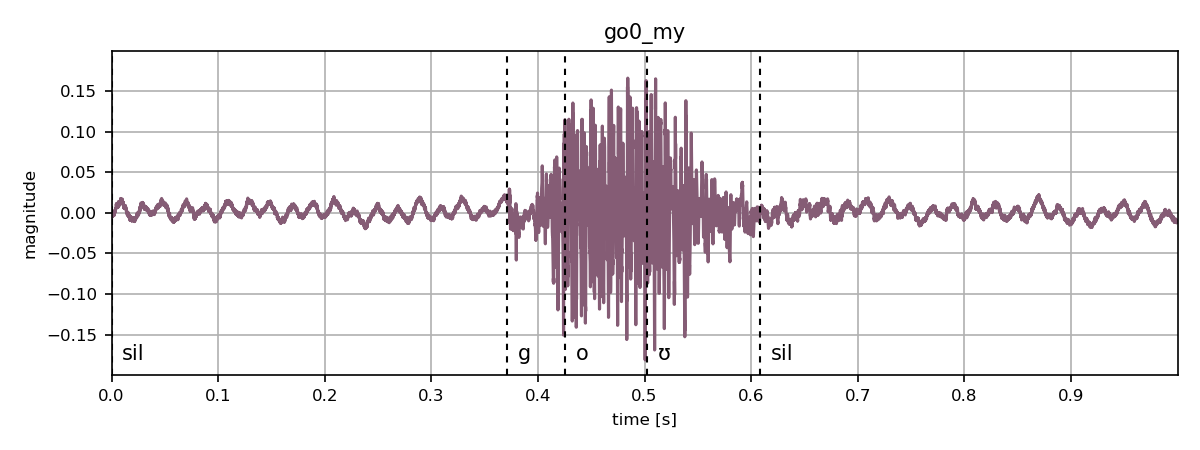
\includegraphics[width=0.45\textwidth]{./3_theory/figs/a1_raw/raw_go0_my}}
  \caption{Raw audio waveform files, recorded and annotated by the author with $f_s=16kHz$ and a simple consumer lavalier microphone.}
  \label{fig:raw_audio_my}
\end{figure}
\FloatBarrier
\noindent
From the raw audio files with annotations, one can observe that and estimate how long a speech command may take in terms of time and see that usually a whole second is too much for a single speech command.
Of course one can pronounce words longer or shorter, but usually in commanding something it is preferred to speak short well pronounced.
If a time interval of 500ms is used to capture a speech command (this time interval is used in the feature extraction for the machine learning), it might happen that not every phonetic letter of the words are captured. For instance this might happen often for words with glottal stops before consonants, as the phoneme \enquote{t} in \enquote{left} or \enquote{right}.
So the input features may only have information of the first phonetics, e.g. \enquote{lef} or \enquote{righ}, but since Key Word Spotting is restricted in its vocabulary, it should be no problem in distinguishing these two words when using a time interval of 500ms.

Another important point is to detect where the onset of the speech command is located on the time axis. It is easy to see in \rfig{raw_audio_my} where the words are starting, but usually not all recordings are as clean as those.
There might be a huge noise level or background noise and it is difficult to find the right onset position for the 500ms time interval with the 1s recordings.
For this Question to answer, it is postponed to the next sections on feature extraction.
At last it should be noted, that the value range in the y-axis of audio recordings strongly depends on the microphone, amplifiers and post processing.
It is naturally that all recording must be normalized to a specific value range, usually $[-1, 1]$.